\documentclass[titlepage = firstcover]{scrartcl}
\usepackage[aux]{rerunfilecheck}
\usepackage{fontspec}
\usepackage[main=ngerman, english, french]{babel}

% mehr Pakete hier
\usepackage{expl3}
\usepackage{xparse}

%Mathematik------------------------------------------------------
\usepackage{amsmath}   % unverzichtbare Mathe-Befehle
\usepackage{amssymb}   % viele Mathe-Symbole
\usepackage{mathtools} % Erweiterungen für amsmath
\usepackage[
  math-style=ISO,    % \
  bold-style=ISO,    % |
  sans-style=italic, % | ISO-Standard folgen
  nabla=upright,     % |
  partial=upright,   % /
]{unicode-math}% "Does exactly what it says on the tin."
\usepackage[section, below]{placeins}

% Laden von OTF-Mathefonts
% Ermöglich Unicode Eingabe von Zeichen: α statt \alpha

\setmathfont{Latin Modern Math}
%\setmathfont{Tex Gyre Pagella Math} % alternativ zu Latin Modern Math
\setmathfont{XITS Math}[range={scr, bfscr}]
\setmathfont{XITS Math}[range={cal, bfcal}, StylisticSet=1]

\AtBeginDocument{ % wird bei \begin{document}
  % werden sonst wieder von unicode-math überschrieben
  \RenewDocumentCommand \Re {} {\operatorname{Re}}
  \RenewDocumentCommand \Im {} {\operatorname{Im}}
}
\usepackage{mleftright}
\setlength{\delimitershortfall}{-1sp}

%Sprache----------------------------------------------------------
\usepackage{microtype}
\usepackage{xfrac}
\usepackage[autostyle]{csquotes}    % babel
\usepackage[unicode, pdfusetitle]{hyperref}
\usepackage{bookmark}
\usepackage[shortcuts]{extdash}
%Einstellungen hier, z.B. Fonts
\usepackage{booktabs} % Tabellen


\title{Wärmeleitfähigkeit}
\author{
  David Gutnikov\\
  \href{mailto:david.gutnikov@udo.edu}{david.gutnikov@udo.edu}
 \and 
  Lasse Sternemann\\
  \href{mailto:lasse.sternemann@udo.edu}{lasse.sternemann@udo.edu}
}
\date{Durchführung am 10.12.2019}


\begin{document}
  \maketitle
  \newpage
  \tableofcontents
  \newpage

  \section{Zielsetzung}
    Mithilfe dieses Versuch sollen die Wärmeleitfähigkeiten für verschiedene Materialien bestimmt werden.

  \section{Theoretische Grundlagen}
    Wärme kann innerhalb eines Körpers durch Konvektion, Wärmestrahlung oder Wärmeleitung transportiert werden.
    Dabei wird Wärmeleitung durch frei bewegliche Elektronen oder Gitterschwingungen, den Phononen, des Materials betrieben.
    In Metallen, welche in diesem Versuch betrachtet, werden geschieht dies haupsächlich durch die freien Elektronen.
    Damit Wärmeleitung stattfindet muss ein Temperaturgradient in dem Körper vorhanden sein.
    Es herrscht ein Temperaturgefälle von einem zum anderen Ende eines Stabes der Dichte $\rho$, der Länge $l$,
    der Querschnittsfläche $A$ und der spezifischen Wärmekapazität $c$ vor. Für die Wärmemenge $dQ$, die im Zeitraum $dt$
    durch $A$ fließt, gilt folgende Formel:
    \begin{equation}
      dQ = -\kappa A \frac{\partial T}{\partial x} dt = j_w A dt
      \label{eqn:dQ}
    \end{equation}
    Wobei $\kappa$ die gesuchte Wärmeleitfähigkeit des Materials und $j_w$ die Wärmestromdichte ist.
    Mit Hilfe der Kontinuitätsgleichung \eqref{eqn:kontinuitätsgl} für lineare Wärmeströme,
    \begin{equation}
        \label{eqn:kontinuitätsgl}
      \frac{\partial T}{\partial t} + \frac{1}{\rho c} \frac{\partial j_w}{\partial x} = 0
    \end{equation}
    ergibt sich beim Einsetzen von $j_w$ die Wärmeleitungsgleichung \eqref{eqn:wärmeleitungsgl}:
    \begin{equation}
        \label{eqn:wärmeleitungsgl}
      \frac{\partial T}{\partial t} = \frac{\kappa}{\rho c} \frac{\partial^2 T}{\partial x^2}
    \end{equation}
    
    \noindent
    Werden lange Stäbe, um die es sich in diesem Versuch handelt, mit einer Periode $T_periode$ erhitzt und geküklt,
    so sieht die Lösung von \eqref{eqn:wärmeleitungsgl}, also die sich ergebende Temperaturwelle wie folgt aus:
    \begin{equation}
      T(x, t) = T_{\text{max}} e^{\sqrt{\frac{\omega \rho c}{2 \kappa}}x} \cos \biggl(\omega t - \sqrt{\frac{\omega \rho c}{2 \kappa}}x \biggr)
    \end{equation}
    \newpage

  \section{Versuchsdurchführung}
    Es werden vier Stäbe gleicher Maße, davon einer aus Aluminium, Edelstahl und zwei aus Messing, auf einer Platine \ref{fig:platine}
    eingespannt, sodass sie mithilfe eines Peltierelementes gleichzeitig an einem Ende erwärmt und gekühlt werden können.
    Es sind je zwei Thermoelemente zu Temperaturmessung in gleichem Abstand an den Stäben angebracht. Die Thermoelemente
    sind mit einem Gerät verbunden, welches die gemessenen Daten in bestimmten Zeitabständen aufnimmt. Die Stäbe müssen
    während den Messungen immer mit einer Wärmeisolierung bedeckt sein, damit die Werte nicht durch äußere Einflüsse
    verfälscht werden. Nach den Messungen soll die Wärmeisolierungentfernt werden, um die Stäbe wieder schneller 
    auf Zimmertemperatur runter zu kühlen.
    \subsection{Statische Methode}
      Hierbei werden die Stäbe so lange erwärmt bis Thermoelement 7 eine Temperatur von ca. 45° anzeigt. Die Spannung
      am Peltierelement beträgt 5V bei maximalem Strom und die Temperaturwerte an den Thermoelementen werden mit einer
      Abtastrate von 5 Sekunden abgenommen.
    \subsection{Dynamische Methode}
      Diese Messungen werden so lange ausgeführt bis eins der Thermoelemente 80° anzeigt, dabei beträgt die Spannung am
      Peltierelement 8V bei maximalem Strom. Bei der ersten Messreihe wird das Peltierelement mit einer Periode von
      80 Sekunden umgestellt, sodass die Stäbe abwechselnd erwärmt und gekühlt werden. Für die zweite Messreihe werden
      die Perioden auf 200 Sekunden verlängert. Dabei wird eine Abtastrate der Messwerte von 2 Sekunden genommen.
    
    \begin{figure}[h]
      \centering
      \label{fig:platine}
      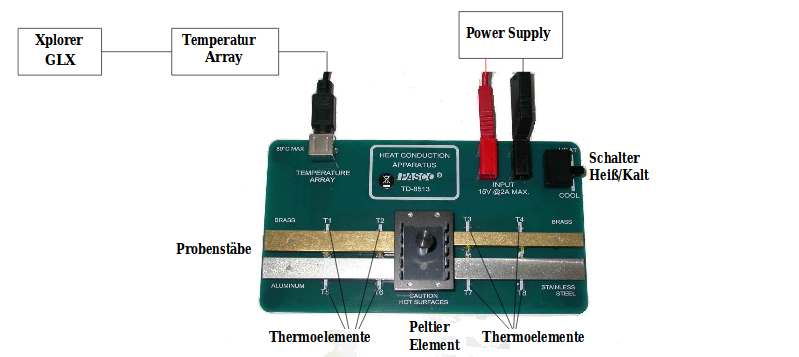
\includegraphics[width = 0.7\linewidth]{Platine.png}
    \end{figure}

    \FloatBarrier

  \section{Auswertung}
    In der Auswertungen wird zur Berechnung von Mittelwerten der Mittelwertssatz \eqref{eqn:Mittelwertssatz} verwendet. Die zugehörige Standardabweichung 
    wird mit Formel \eqref{eqn:Stanni} berechnet und für Werte die von fehlerbehafteten Größen abhängen, wird die Gaußsche Fehlerfortpflanzung 
    \eqref{eqn:Gauß} verwendet.
    \begin{equation}
      \overline{x} = \frac{1}{N} \cdot \sum_{i=1}^{N} x_i
      \label{eqn:Mittelwertssatz}
    \end{equation}

    \begin{equation}
      \Delta \overline{x} = \sqrt{\frac{1}{n(n-1)} \cdot \sum_{i=1}^n (x_i - \overline{x})^2}
      \label{eqn:Stanni}
    \end{equation}
    
    \begin{equation}  
      \Delta f = \sqrt{\sum_{i=1}^N \left(\frac{df}{dy_i} \cdot \Delta y_i \right)}
      \label{eqn:Gauß}
    \end{equation}  




    %Graphen
  \subsection{Statische Methode}
  \begin{figure}
    \centering
    \caption{In der Grafik sind die Temperaturverläufe der 4 verschiedenen Messplatten zu sehen.}
    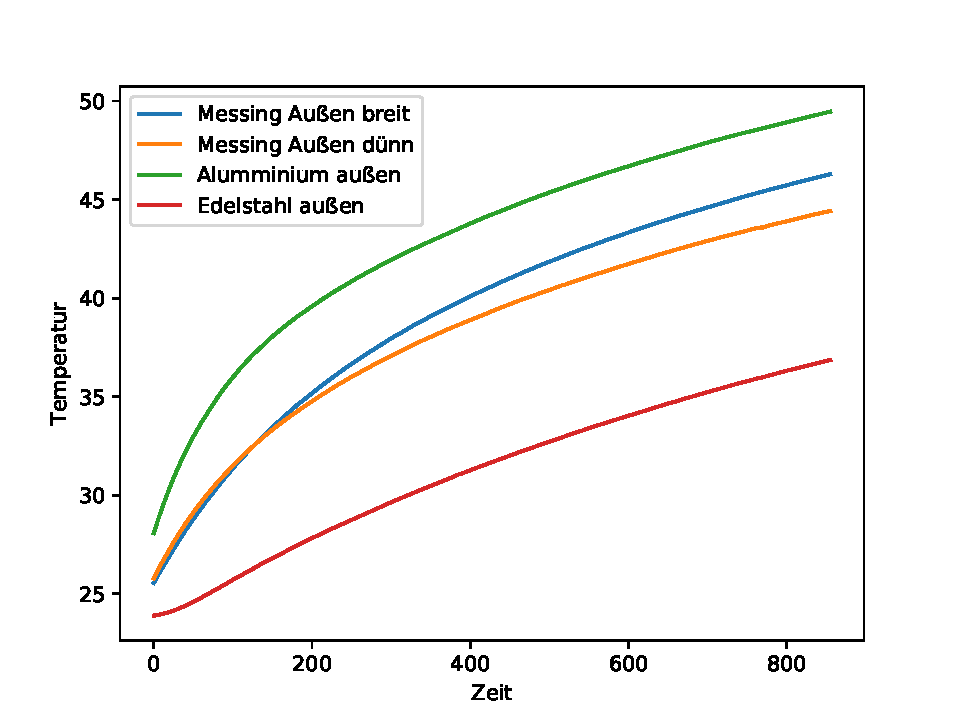
\includegraphics{Tstatisch.pdf}
    \label{fig:Tstat}
  \end{figure}

  Wie in Grafik \ref{fig:Tstat} zu sehen ist, steigen die äußeren Temperaturen von Aluminium und den beiden Messingplatten zu Beginn sehr stark an. Ab 
  einer Dauer von etwa 150s schwacht der Temperaturanstieg hingegen ab und die Temperatur scheint gegen einen Maximalwert zu laufen, der mit der durchgeführten
  Messung jedoch nicht erreicht wurde. Aluminium scheint dabei am wärmsten zu werden und auch den stärksten Temperaturanstieg zu haben. Bei den beiden
  Messingplatten ist zu Beginn ein beinahe gleicher Anstieg der Temperatur zu erkennen. Nach ca. 160s trennen sich jedoch die Kurven und der breitere Stab läuft
  gegen eine leicht höhere Temperatur. Im Vergleich zu den anderen 3 Stäben wirkt der Temperaturanstieg des Edelstahlstabs beinahe linear und zugleich sehr schwach.
  Dies zeigt sich auch an den Temperaturen, die die Platten nach 700s inne haben \ref{tab:700s}. Nach diesen Werten hat die Aluminiumplatte die beste Wärmeleitung,
  die breite Messingplatte die zweitbeste, die dünne Messingplatte die drittbeste und die Edelstahlplatte die schlechteste.

  \begin{table}[h]
    \centering
    \caption{In der Tabelle sind die Temperaturen der einzelnen Messplatten zum Zeitpunkt t=700S angegeben.}
    \label{tab:700s}
    \begin{tabular}{c c}
      \toprule
      {Messplate} & {$T_{\text{700s}} [\text{°C}]$} \\
      \midrule 
      Aluminium & 47,90 \\
      Edelstahl & 35.24 \\
      Messing (dünn) & 42.91 \\
      Messing (breit) & 44.62 \\
      \bottomrule
    \end{tabular}
  \end{table}


  Nun kann nach Umstellen von Gleichung \eqref{eqn:dQ} der Wärmestrom in den Platten wie folgt berechnet werden:
  \begin{equation*}
    \frac{dQ}{dT} = - \kappa \cdot A \cdot \frac{\partial T}{\partial x}
  \end{equation*}
  Dabei steht $\kappa$ für die Wärmeleitfähigkeit des Materials, A für dessen Querschnittsfläche, $\partial T$ für die Temperaturdifferenz zwischen den zwei 
  Punkten und $\partial x$ für den Abstand der zwei Punkte, der bei diesem Experiment immer 3cm beträgt.
  \begin{align*}
    A_{\text{Aluminium}} =& 4,8 \cdot 10^{-5} m^2 \qquad    \kappa_{\text{Aluminium}}=220 \: \frac{W}{mK}\\
    A_{\text{Edelstahl}} =& 4,8 \cdot 10^{-5} m^2 \qquad    \kappa_{\text{Edelstahl}}=21 \: \frac{W}{mK}\\
    A_{\text{Messing breit}} =& 4,8 \cdot 10^{-5} m^2 \qquad \kappa_{\text{Messing}}=105  \: \frac{W}{mK}  \\
    A_{\text{Messing dünn}} =& 2,8 \cdot 10^{-5} m^2 \qquad \kappa_{\text{Messing}}=105  \: \frac{W}{mK}  \\
  \end{align*}

  Mit den oben gegebenen Rahmenwerten und den Messwerten lassen sich folgende Wärmeströme berechnen.

  \begin{table}[h]
    \centering
    \caption{Der Wärmestrom in den verschiedenen Metallplatten zu 5 verschiedenen Zeitpunkten}
    \label{tab:Wärmeströme}
    \begin{tabular}{c c c c}
      \toprule
      {Platte} & {t [s]} & {$T_{\text{diff}}$} & {Wärmestrom $\frac{dQ}{dT} \: [W \cdot 10^{-4}]$} \\
      \midrule
      Aluminium &    145      &      1,60       &     -66,00      \\ 
                &    295      &      1,34       &     -78,81      \\
                &    445      &      1,30       &     -81,23      \\
                &    595      &      1,29       &      -81,86     \\
                &    745      &      1,29       &      -81,86     \\
      Edelstahl &    145      &      7,60       &     -1,33      \\ 
                &    295      &      7.97       &     -1,26      \\
                &    445      &      8,09       &     -1,25      \\
                &    595      &      8,13       &     -1,24      \\
                &    745      &      8,15       &     -1,24      \\
  Messing breit &    145      &      3,07       &     - 16,42     \\ 
                &    295      &      2,66       &     - 18,95     \\
                &    445      &      2,54       &     - 19,85     \\
                &    595      &      2,50       &     - 20,16     \\
                &    745      &      2,47       &     - 20,40     \\
   Messing dünn &    145      &      3,28       &     - 8,96     \\ 
                &    295      &      2,99       &     - 9,83     \\
                &    445      &      2,95       &     - 9,97     \\
                &    595      &      2,98       &     - 9,87     \\
                &    745      &      3,01       &     - 9,77     \\
      \bottomrule
    \end{tabular}    
  \end{table}

  \newpage

  \begin{figure}
    \centering
    \caption{In der Grafik sind die Verläufe der Temperaturdifferenz zwischen dem inneren und äußeren Messpunkt von Edelstahl
             und Messing zu sehen.}
    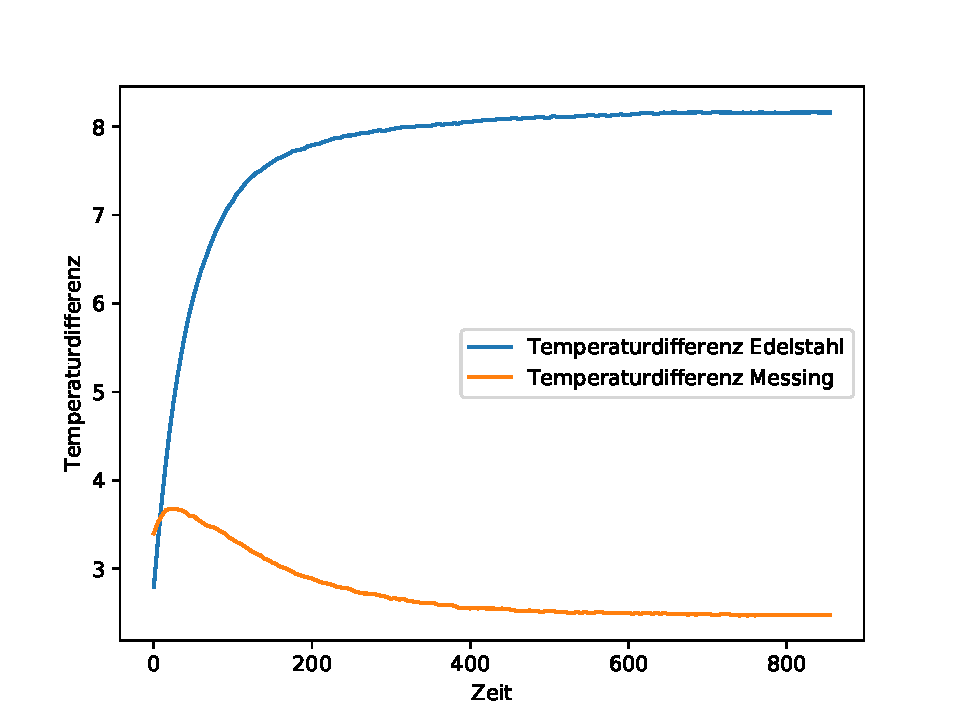
\includegraphics{diffstatisch.pdf}
    \label{fig:diffstat}
  \end{figure}

  

  Beim Vergleich der beiden Graphen aus Abbildung \ref{fig:diffstat} fällt auf, dass die Temperaturdifferenz auf der Edelstahlplatte immer größer wird und dann nach ca 170s beginnt gegen einen
  Wert um die 8 °C zu laufen. Auch die Temperaturdifferenz auf der Aluminiumplatte läuft gegen einen Wert. Hier sinkt die Temperaturdifferenz jedoch und läuft
  gegen eine Temperaturdifferenz zwischen 3  und 2 °C. Auffällig ist, dass die Temperaturdifferenz auf der Edelstahlplatte weitaus schneller steigt, als die 
  auf der Aluminiumplatte sinkt. Das Verhalten der beiden Kurven deutet auf die im Vergleich zum Aluminium schlechte Wärmeleitfähigkeit des Edelstahls hin.

  \FloatBarrier

  \newpage

  \subsection{Dynamische Methode}
  Um die Amplitude und Phasenverschiebung zwischen den beiden Temperaturverläufen zu finden, werden zwei verschiedene Methoden verwendet. Zur Bestimmung
  der Phasendifferenz werden die Zeitpunkte ausgelesen, bei denen die Kurven ihre Minima haben. Die Phasendifferenz ergibt sich dann über den Zeitunterschied.
  Zur Bestimmung der Amplitude muss zuerst der Untergund abgezogen werden. Dazu wird dieser mit einem Polynom 4. Grades modelliert. Nun kann die Temeperatur-
  welle erneut, nun jedoch ohne Untergund gezeichnet werden. In dieser Grafik sieht man nun deutlich die Amplitude und kann diese berechnen, indem man die 
  Differenz der gemittelten Maxima sowie Minima berechnet und diese dann durch 2 teilt. Bei späteren Berechnungen werden folgende Werte und x = 0,03m verwendet:

  \begin{align*}
    \rho_{\text{Aluminium}} =& 2800 \: \frac{kg}{m^3} \qquad    c_{\text{Aluminium}}=830 \: \frac{J}{kgK}\\
    \rho_{\text{Edelstahl}} =& 8000 \: \frac{kg}{m^3} \qquad    c_{\text{Edelstahl}}=400 \: \frac{J}{kgK}\\
    \rho_{\text{Messing}} =& 8520 \: \frac{kg}{m^3} \qquad c_{\text{Messing}}=385  \: \frac{J}{kgK}  \\
  \end{align*}



  Die Phasendifferenzen finden sich in Tabelle \ref{tab:Phasen} und zu den Werten wird die Standardabweichung des Mittelwerts berechnet \eqref{eqn:Stanni}.

    \subsubsection{Aluminium}
    Über das beschriebene Vorgehen ergibt sich hier für die Phasendifferenz:
    \begin{equation*}
      \Delta t = (5,25 \pm 0,17) s
    \end{equation*}
      \begin{figure}[h]
        \centering
        \caption{In der Grafik sind die Temperaturwellen und der durch die Minima modellierte Untergund dargestellt.}
        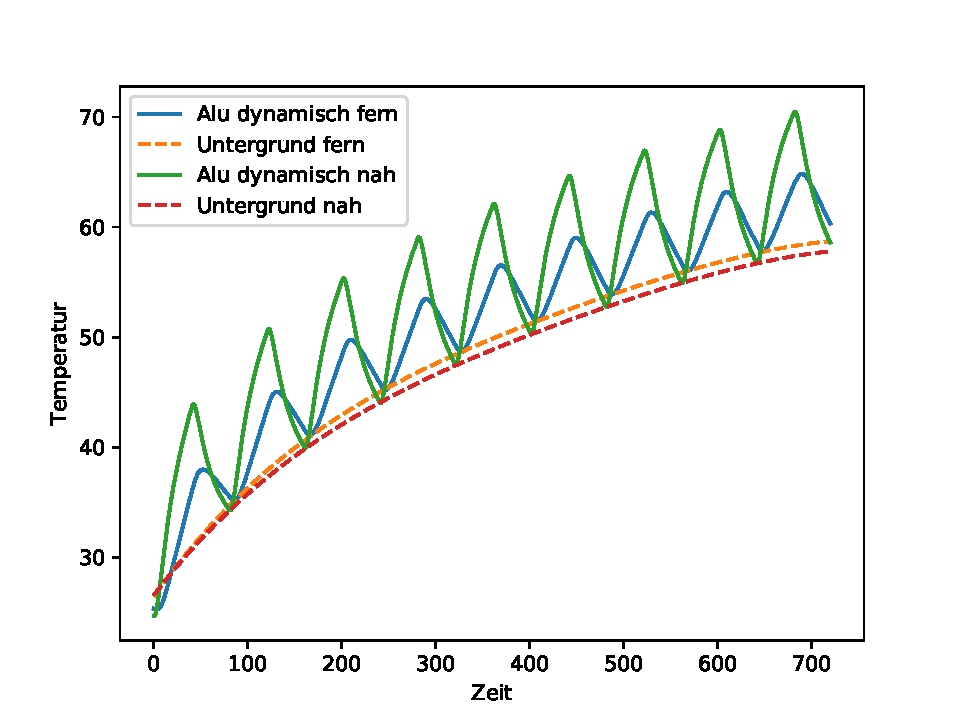
\includegraphics{dynamischalu1.pdf}
        \label{fig:dynamischalu}
      \end{figure}

    Nach Ausfiltern des Untergrunds ergeben sich die zwei neuen Grafiken, aus denen die Amplituden bestimmt werden. 

      \begin{figure}[h]
        \centering
        \caption{In der Grafik ist die Wellenfunktion am fernen Messpunkt zu sehen, nachdem der Untergund abgezogen wurde.}
        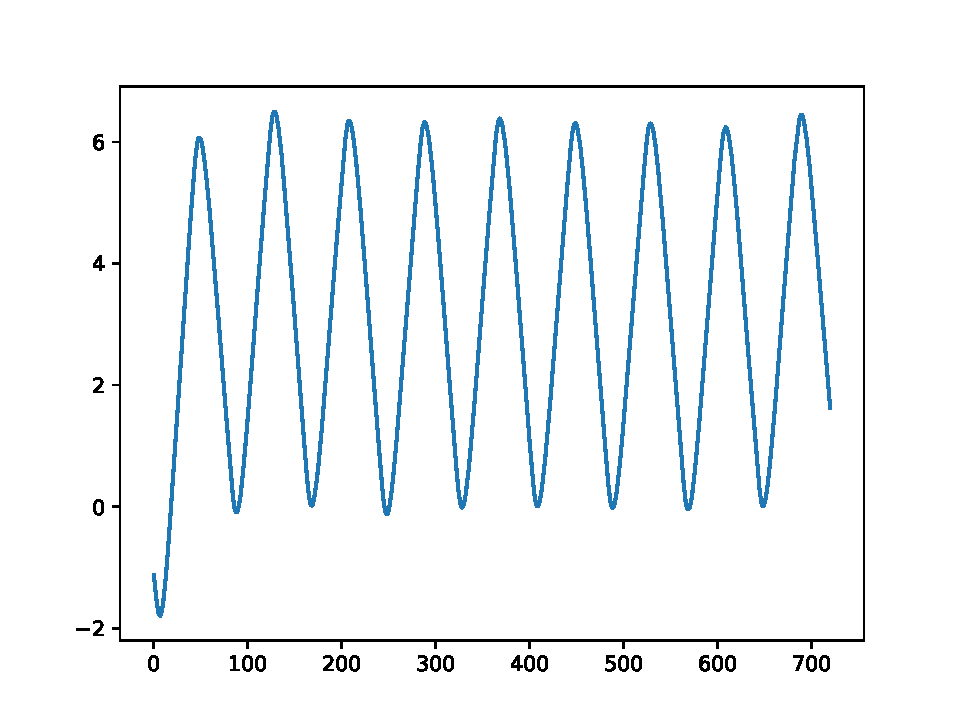
\includegraphics{AmpAluFern.pdf}
        \label{fig:AmpAluFern}
      \end{figure}

      \begin{figure}[h]
        \centering
        \caption{In der Grafik ist die Wellenfunktion am nahen Messpunkt zu sehen, nachdem der Untergund abgezogen wurde.}
        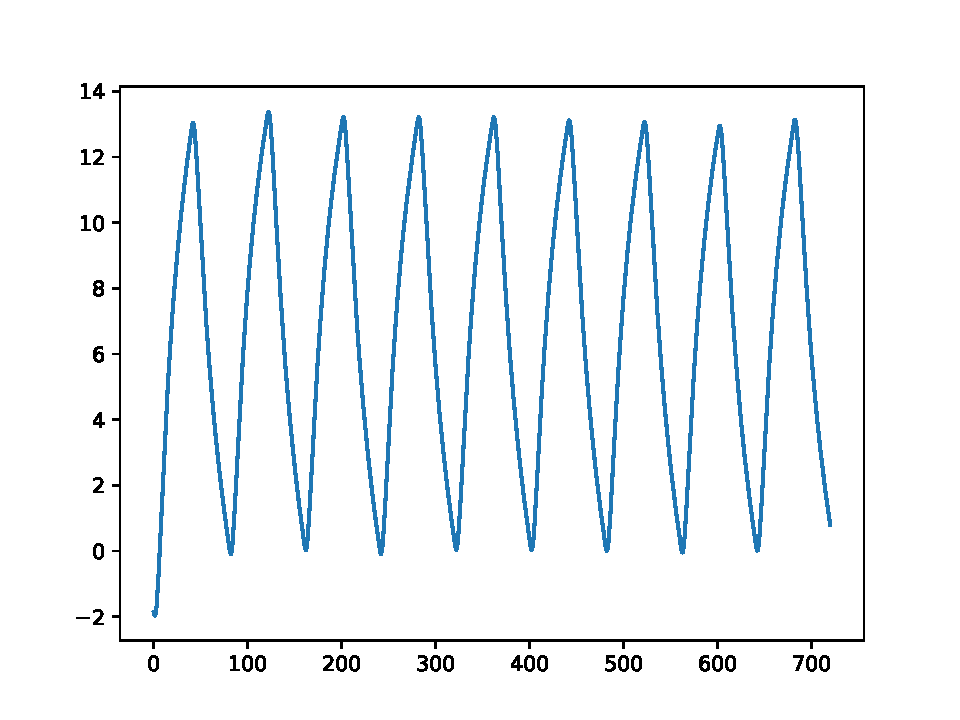
\includegraphics{AmpAluNah.pdf}
        \label{fig:AmpAluNah}
      \end{figure}

    Es ergeben sich folgende gemittelte Minima und Maxima:

    \begin{table}[h]
      \centering
      \caption{Die Maxima und Minima der Welle am nahen und fernen Messpunkt für Aluminium}
      \label{tab:AmplitudeAlu}
      \begin{tabular}{c c c c c}
        \toprule
        {Extrema} & $Maxima_{\text{Nah}}$ & $Minima_{\text{Nah}}$ & $Maxima_{\text{Fern}}$ & $Minima_{\text{Fern}}$ \\
        \midrule
        Extrema       & 13,04&0,1      &6,50 & 0,09 \\
                & 13,38&-0,03     &6,35 & 0,12 \\
                & 13,21& 0,10     &6,32 & 0,02 \\
                & 13,21& -0,03    &6,38 & 0,01 \\
                & 13,21& -0,03    &6,31 &- \\
                & 13,11& -0,0006  &6,30 &- \\
                & 13,06& 0,05     &6,24 &- \\
                & 12,94& -        &-    &- \\
                & 13,13& -        &-    &- \\
  $\overline{Extremum}$ & 13,14 & 0,024  &   6,34  & 0,06 \\
  $\Delta \overline{Extremum}$ & $\pm 0,05 $ & $\pm 0,02$  & $\pm 0,04$  & $\pm 0,03$ \\

        \bottomrule
      \end{tabular}   
    \end{table}
    Nun wird die Amplitude aus den gemittelten Extrema berechnet. Der Fehler ergibt sich aus den vorherigen Fehlern der Extrema.
    \begin{align*}
      A_f =& (6,4 \pm 0,3) °C\\
      A_n =& (13,2 \pm 0,6) °C
    \end{align*}

    Nun muss nur noch die Wärmeleitfähigkeit über Formel \eqref{eqn:wärmeleitungsgl} und der Fehler über folgende Fehlerfortpflanzung berechnet werden.
    \begin{equation*}
      \Delta \kappa = \sqrt{(\frac{\rho c x^2}{2 \Delta t A_f ln^2(\frac{A_n}{A_f})}\cdot \Delta A_f)^2 + (\frac{-\rho c x^2}{2 \Delta t A_n ln^2(\frac{A_n}{A_f})}\cdot \Delta A_n)^2 + (\frac{-\rho c x^2}{2 \Delta t^2 ln(\frac{A_n}{A_f})}\cdot \Delta(\Delta f))^2}
    \end{equation*}
    So ergibt sich:
    \begin{equation*}
      \kappa = (275 \pm 27) \; \frac{W}{mK}
    \end{equation*}
    Dieser berechnete Wert weicht zum Literaturwert[2] von 220 $\frac{W}{mK}$ um 20 \% ab.

  \FloatBarrier

  \newpage



    \subsubsection{Messing}
    Über das beschriebene Vorgehen ergibt sich hier für die Phasendifferenz:
    \begin{equation*}
      \Delta t = (7,9 \pm 0,5) s
    \end{equation*}
    \begin{figure}[h]
      \centering
      \caption{In der Grafik sind die Temperaturwellen und der durch die Minima modellierte Untergund dargestellt.}
      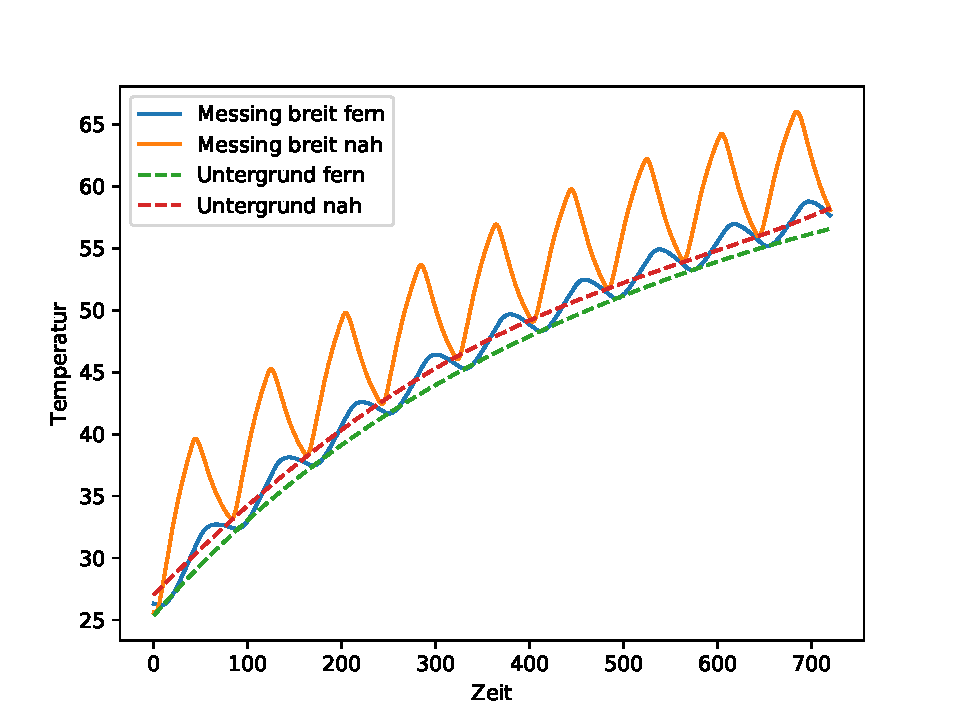
\includegraphics{dynamischmessingbreit.pdf}
      \label{fig:dynamischmes}
    \end{figure}

  Nach Ausfiltern des Untergrunds ergeben sich wieder die zwei neuen Grafiken, aus denen die Amplituden bestimmt werden. 

    \begin{figure}[h]
      \centering
      \caption{In der Grafik ist die Wellenfunktion am fernen Messpunkt zu sehen, nachdem der Untergund abgezogen wurde.}
      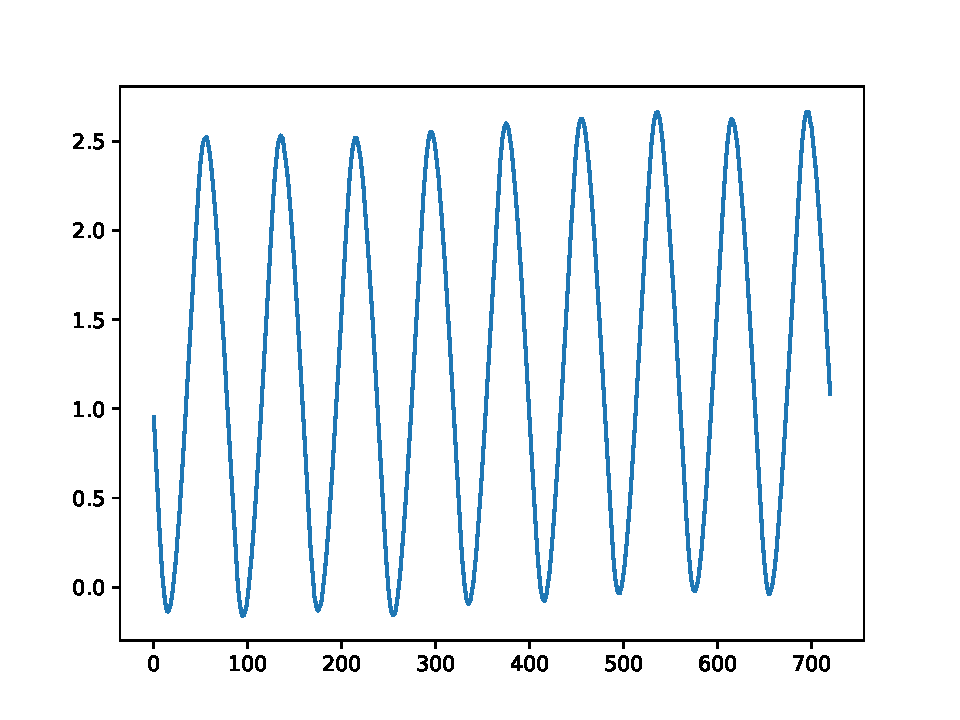
\includegraphics{AmpMesbreitFern.pdf}
      \label{fig:AmpMesFern}
    \end{figure}

    \begin{figure}[h]
      \centering
      \caption{In der Grafik ist die Wellenfunktion am nahen Messpunkt zu sehen, nachdem der Untergund abgezogen wurde.}
      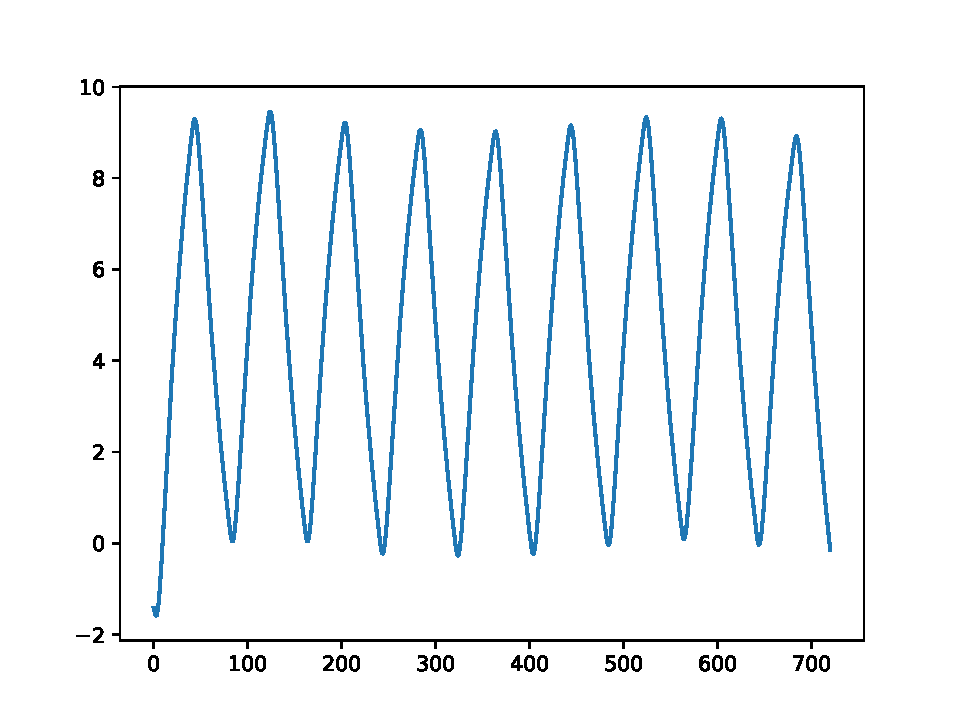
\includegraphics{AmpMesbreitNah.pdf}
      \label{fig:AmpMesNah}
    \end{figure}

  Es ergeben sich folgende gemittelte Minima und Maxima:

  \begin{table}[h]
    \centering
    \caption{Die Maxima und Minima der Welle am nahen und fernen Messpunkt für Messing}
    \label{tab:AmplitudeMes}
    \begin{tabular}{c c c c c}
      \toprule
      {Extrema} & $Maxima_{\text{Nah}}$ & $Minima_{\text{Nah}}$ & $Maxima_{\text{Fern}}$ & $Minima_{\text{Fern}}$ \\
      \midrule
      Extrema &9,29 &-0,05 &2,52 &0,16 \\
              &9,46 &-0,05 &2,53 &0,13 \\
              &9,21 &0,23  &2,52 &0,16 \\
              &9,06 &0,27  &2,55 &0,09 \\
              &9,02 &0,23  &2,60 &0,08 \\
              &9,16 &0,04  &2,63 &0,03 \\
              &9,34 &-0,09 &2,66 &0,02 \\
              &9,31 & -    &2,62 &0,04 \\
              &8,92 & -    &-    &-    \\
  $\overline{Extremum}$ & 9,20 & 0,08  &   2,58  & 0,09 \\
  $\Delta \overline{Extremum}$ & $\pm 0,06 $ & $\pm 0,06$  & $\pm 0,02$  & $\pm 0,02$ \\

      \bottomrule
    \end{tabular}   
  \end{table}
  Nun wird die Amplitude wieder aus den gemittelten Extrema berechnet. Der Fehler ergibt sich aus den vorherigen Fehlern der Extrema.
  \begin{align*}
    A_f =& (1,33 \pm 0,04) °C\\
    A_n =& (4,64 \pm 0,12) °C
  \end{align*}

  Zuletzt muss wieder die Wärmeleitfähigkeit über Formel \eqref{eqn:wärmeleitungsgl} und der Fehler über dieselbe Fehlerfortpflanzung berechnet werden.
  %\begin{equation*}
  %  \Delta \kappa = \sqrt{(\frac{\rho c x^2}{2 \Delta t A_f ln^2(\frac{A_n}{A_f})}\cdot \Delta A_f)^2 + (\frac{-\rho c x^2}{2 \Delta t A_n ln^2(\frac{A_n}{A_f})}\cdot \Delta A_n)^2 + (\frac{-\rho c x^2}{2 \Delta t^2 ln(\frac{A_n}{A_f})}\cdot \Delta(\Delta f))^2}
  %\end{equation*}
  So ergibt sich:
  \begin{equation*}
    \kappa = (152 \pm 21) \; \frac{W}{mK}
  \end{equation*}
  Der berechnete Wert weicht zum Literaturwert[3] von 105 $\frac{W}{mK}$ um 30,92 \% ab.

  \FloatBarrier

  \newpage

  \subsubsection{Edelstahl}
  Wieder das beschriebene Vorgehen angewandt, ergibt sich hier für die Phasendifferenz:
  \begin{equation*}
    \Delta t = (31 \pm 4) s
  \end{equation*}
  \begin{figure}[h]
    \centering
    \caption{In der Grafik sind die Temperaturwellen und der durch die Minima modellierte Untergund dargestellt.}
    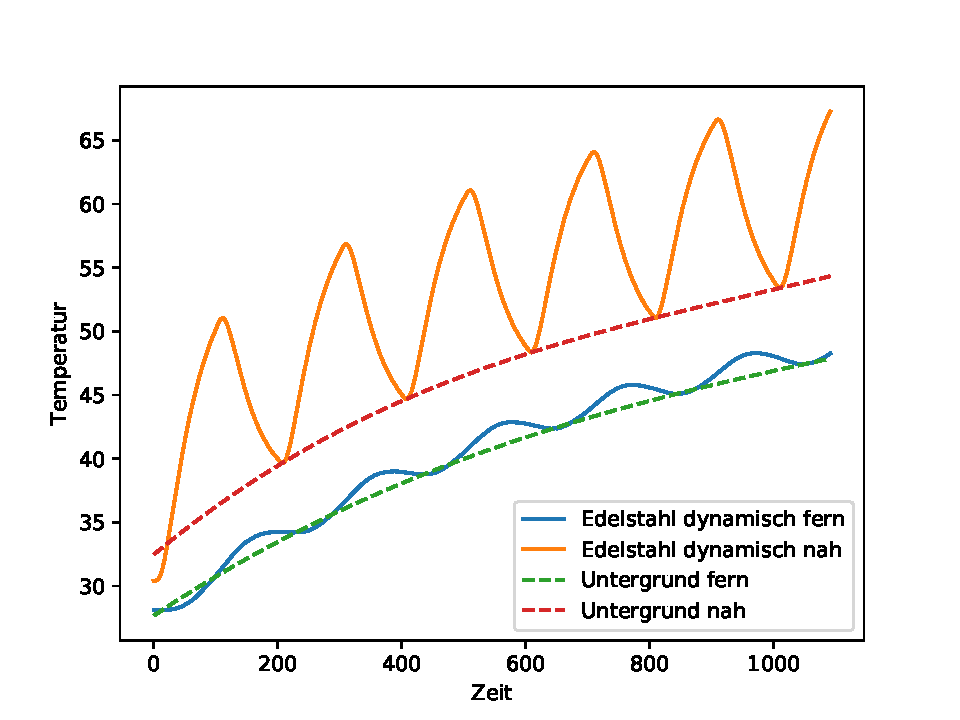
\includegraphics{dynamischstahl2.pdf}
    \label{fig:dynamischstahl}
  \end{figure}

  Die Graphen zur Bestimmung der Amplituden werden analog zu den vorherigen Fällen gebildet. 

  \begin{figure}[h]
    \centering
    \caption{In der Grafik ist die Wellenfunktion am fernen Messpunkt zu sehen, nachdem der Untergund abgezogen wurde.}
    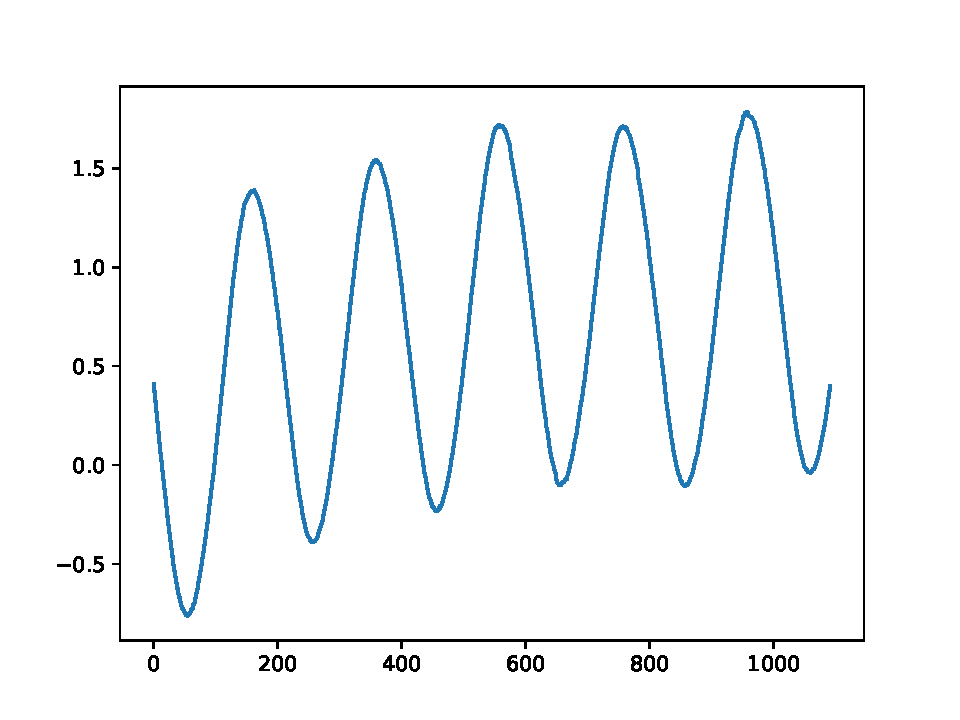
\includegraphics{AmpStahlFern.pdf}
    \label{fig:AmpStahlFern}
  \end{figure}

  \begin{figure}[h]
    \centering
    \caption{In der Grafik ist die Wellenfunktion am nahen Messpunkt zu sehen, nachdem der Untergund abgezogen wurde.}
    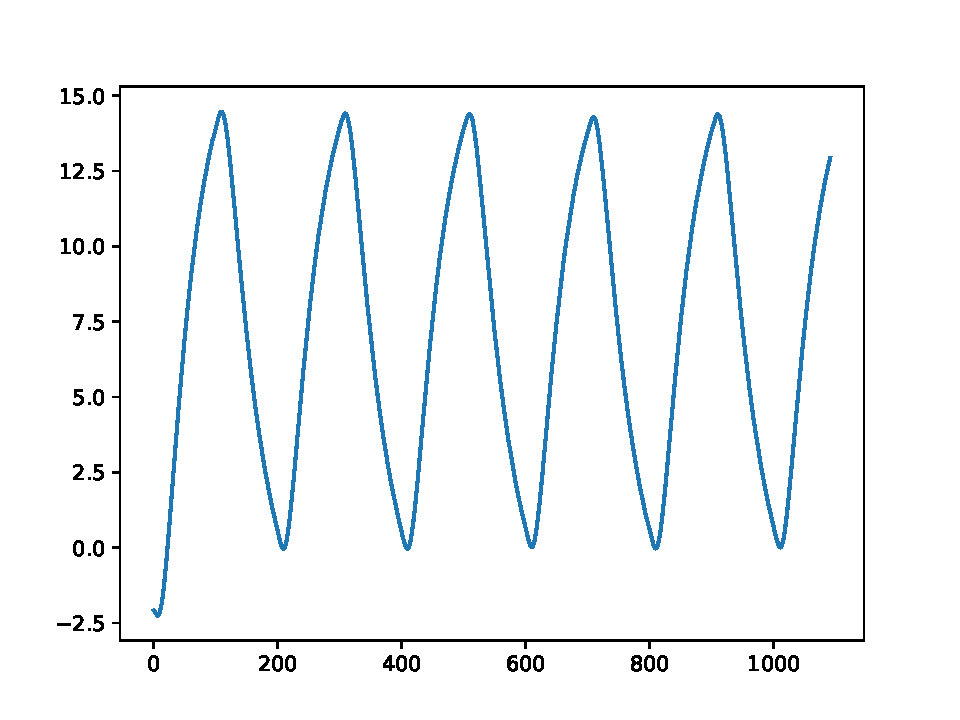
\includegraphics{AmpStahlNah.pdf}
    \label{fig:AmpStahlNah}
  \end{figure}

  Es ergeben sich folgende gemittelte Minima und Maxima:

  \begin{table}[h]
  \centering
  \caption{Die Maxima und Minima der Welle am nahen und fernen Messpunkt für Edelstahl}
  \label{tab:AmplitudeMes}
  \begin{tabular}{c c c c c}
    \toprule
    {Extrema} & $Maxima_{\text{Nah}}$ & $Minima_{\text{Nah}}$ & $Maxima_{\text{Fern}}$ & $Minima_{\text{Fern}}$ \\
    \midrule
    Extrema &14,47  &0,03  &1,72  &0,04 \\
            &14,41  &0,03  &1,71  &0,11 \\
            &14,39  &-0,03 &1,79  &0,10 \\
            &14,29  &0,02  &-     &- \\
            &14,38  &-0,01 &-     &- \\
            &-      &-     &-     &- \\
            &-      &-     &-     &- \\
            &-      &-     &-     &- \\
            &-      &-     &-     &- \\
  $\overline{Extremum}$ & 14,390 & 0,012  &   1,740  & 0,083 \\
  $\Delta \overline{Extremum}$ & $\pm 0,030 $ & $\pm 0,013$  & $\pm 0,024$  & $\pm 0,022$ \\

    \bottomrule
  \end{tabular}   
  \end{table}
  Die Amplitude und ihr Fehler ergeben sich ebenfalls wie bei den anderen Fällen.
  \begin{align*}
  A_f =& (0,91 \pm 0,05) °C\\
  A_n =& (7,20 \pm 0,05) °C
  \end{align*}

  Wieder muss nur noch die Wärmeleitfähigkeit über Formel \eqref{eqn:wärmeleitungsgl} und der Fehler über die bekannte Fehlerfortpflanzung berechnet werden.
  %\begin{equation*}
  %\Delta \kappa = \sqrt{(\frac{\rho c x^2}{2 \Delta t A_f ln^2(\frac{A_n}{A_f})}\cdot \Delta A_f)^2 + (\frac{-\rho c x^2}{2 \Delta t A_n ln^2(\frac{A_n}{A_f})}\cdot \Delta A_n)^2 + (\frac{-\rho c x^2}{2 \Delta t^2 ln(\frac{A_n}{A_f})}\cdot \Delta(\Delta f))^2}
  %\end{equation*}
  So ergibt sich:
  \begin{equation*}
  \kappa = (22,5 \pm 2,4) \; \frac{W}{mK}
  \end{equation*}
  Dieser berechnete Wert weicht zum Literaturwert [2] von 21 $\frac{W}{mK}$ um 7,14 \% ab.

  \FloatBarrier

  \subsection{Diskussion}
   Beim Vergleich der bestimmten Wärmeleitfähigkeiten mit den Literaturwerten fällt auf, dass die Messung gut genug war, um sie durch die Literaturwerte zu
   verifizieren. Besonders der gemessenen Wert von Edelstahl weicht nur sehr gering vom Literaturwert ab. Auch die gemessenen Graphen geben das zu erwartende
   Bild wieder. So zeigt sich beim Vergleich der Temperaturen bei der statischen Methode, dass die Materialien abhängig von ihrer Wärmeleitfähigkeit
  unterschiedlich schnell und stark die Temperatur leiten. Auch die Graphen zur Temperaturdifferenz bestätigen die Literaturwerte der Wärmeleitfähigkeiten, da
  sie zeigen, dass Materialien mit einer hohen Wärmeleitfähigkeit die Temperaturdifferenz schnell ausgleichen können, während diese bei Materialien mit geringer
  Wärmeleitfähigkeit, in diesem Fall Edelstahl, nicht in der Lage sind die Temperaturdifferenz überhaupt auszugleichen.


  \subsection{Anhang}
        \begin{table}[h]
          \centering
          \caption{Die einzelnen Phasendifferenzen, sowie die Gemittelte.}
          \label{tab:Phasen}
          \begin{tabular}{c c c c}
            \toprule
            {Phasendifferenz} & {Aluminium} & {Edelstahl} & {Messing breit}\\
            \midrule
            $\Delta t$      & 5     & 21    & 6 \\
                            & 5     & 28    & 7 \\
                            & 5     & 32    & 7 \\
                            & 5     & 36    & 7 \\
                            & 5     & 38    & 9 \\
                            & 5     & -     & 9 \\
                            & 6     & -     & 9 \\
                            & 6     & -     & 9 \\
      $\overline{\Delta t}$ & 5,25  & 31    & 7,875 \\
            \bottomrule
          \end{tabular}
        \end{table}


  \subsection{Literaturverzeichnis}
        [1] \textit{Versuchsanleitung V204 - Wärmeleitung von Metallen.} TU Dortmund, 2019 \newline
        [2] H. Recknagel, E. Sprenger, K. Albers: \textit{Recknagel - Taschenbuch für Heizung + Klimatechnik. 77. Ausgabe} \newline
        [3] P. Kurzweil, B. Frenzel, F. Gebhard: \textit{Physik Formelsammlung. 4. Auflage}

    
\end{document}